\chapter{Analyse} %Louisa
Um die Anforderungen für diese Studienarbeit aufstellen zu können, muss eine Analysephase basierend auf die Motivation durchgeführt werden. In der Analysephase werden relevante Anforderungen an das innerhalb dieser Arbeit erarbeitende System evaluiert.
\section{Analysephase} \label{sec:Anforderungen}
Basierend auf die Motivation wird analysiert, welche Parameter die Qualität eines Raumes beeinflussen. Neben der reinen Beeinflussung der Raumqualität, müssen die Parameter zudem untersucht werden auf die Sinnhaftigkeit einer Kontrolle der Werte und einer Messbarkeit der Werte.\\
Die Innenraumklimatologie beschäftigt sich mit den Einflussfaktoren auf das Innenraumklima. Dabei werden chemische, biologische, wie auch physikalische Faktoren betrachtet. Ziel der Innenraumklimatologie ist es ein optimales Wohn- und Arbeitsumfeld im Innenbereich zu ermöglichen \cite{raumluft:Innenraumklimatologie}. Bei einer optimalen Umgebung wird nachweislich die Behaglichkeit gesteigert, sowie die Leistungsfähigkeit \cite{Raumklimatechnik}. Schlechte Raumluft kann zudem gesundheitliche Beeinträchtigungen hervorrufen \cite{raumluft:InnenluftqualitaetundGesundheit}. Beeinflussende Parameter müssen für eine sinnvolle Raumanalyse in ihrer Gesamtheit betrachtet werden.\\
Innerhalb dieser Arbeit wurden als repräsentative Parameter für das Raumklima Temperatur, Luftfeuchtigkeit, Kohlenstoffdioxid (kurz CO\textsubscript{2}) und Kohlenstoffmonoxid (kurz CO) ausgewählt. Diese Werte bilden eine Grundlage für eine generelle Raumüberprüfung. Es wurde sich auf diese fünf Werte beschränkt um eine allgemeine umfassende Raumkontrolle zu bewerkstelligen. Schadstoffe in der Raumluft können sehr stark von Wohngebiet und verwendete Materialien abweichen. Bei einem genaueren Verdacht auf einen Schadstoff müssen die verwendeten Sensoren entsprechend angepasst werden.\\
Neben der Erfassung von den repräsentativen Parametern für das Raumklima sollten noch repräsentative Aktionen in die spätere Auswertung mit einfließen. Es muss erkannt werden, ob und wie lange eine Luftzufuhr durch Fenster oder Türen öffnen stattgefunden hat. Auch Menschen, die sich in einem Raum aufhalten, beeinflussen ihre Umgebung. So trägt der Mensch zum einen zu einer Veränderung der Luftfeuchtigkeit bei, durch die Atmung und die Feuchteabgabe durch die Haut). Zum anderen gibt ein Mensch Gase, wie CO\textsubscript{2} oder andere Schadstoffe, an seine Umgebung ab \cite{raumluft:Luftmengen}. Es sollte aus diesen Gründen erkannt werden, ob sich ein Mensch gerade im Raum aufhält und dadurch diesen beeinflusst.\\
\section{Anforderungen}
Innerhalb dieser Arbeit wurden auf Grundlage der Analyse die Anforderungen an das System gestellt. Die Anforderungen wurden in funktionale und nicht-funktionale Anforderungen unterteilt. Als Kernaufgabe des Systems steht die Verknüpfung von Sensoren mit Akteuren. Dafür ist eine Erfassung und Kontrolle der Sensordaten, sowie die anschließende Verarbeitung der Daten um Akteuren Handlungsaufforderungen mitzuteilen, notwendig. Dem späteren Anwender soll das System eine möglichst optimale Unterstützung bei der Kontrolle der Raumbedingungen ermöglichen. Die Anforderungen wurden in drei verschiedene Kategorien aufgeteilt: 1 - Must haves, 2 - Should Haves und 3 - Could Haves. Die Einteilung in diese Kategorien ist für die Umsetzung hilfreich. In der Tabelle \ref{tab:anforderungen} sind die Anforderungen aufgezeigt. Eine detailliertere Auflistung aller Anforderungen mit Beschreibung sind dem Anhang zu entnehmen.\\

\begin{tabularx}{\textwidth}{|l|X|X|l|l|}
	\toprule
	\textbf{ID-Kürzel} & \textbf{Anforderung} & \textbf{Beschreibung} & \textbf{Prio} & \textbf{Abhängig von} \\
	\hline
	\endhead
	\hline
	\caption{Anforderungen}
	\label{tab:anforderungen}
	\endfoot
	\multicolumn{5}{|l|}{F-00 Allgemein}\\
	\hline
	F-00.1 & Raspberry Pi & Eine Komponente des Systems ist ein Raspberry Pi. & 1 & \\
	F-00.2 & Grafische Benutzerschnittstelle & Das System stellt eine grafische Benutzerstelle bereit. & 1 & \\
	F-00.3 & Sensoren & Es werden Sensoren zur Datenerfassung genutzt. & 1 & \\
	F-00.4 & Akteure & Es werden Akteure an das System angeschlossen. & 3 & \\
	\hline
	\multicolumn{5}{|l|}{F-10 Daten erfassen - Raumbedingungen}\\
	\hline
	F-10.1   & Kamera & Es wird das Kamera Modul des Raspberry Pis genutzt. & 1 & F-00.4\\
	F-10.1.1 & Live-Übertragung & Es wird eine Live-Übertragung des Kamerabildes übertragen. & 1 & F-10.2 \\
	F-10.1.2 & Bewegung & Es können Bewegungen über die Kamera erkannt werden. & 1 & F-10.2 \\
	F-10.2 & Luftfeuchtigkeit & Es kann die Luftfeuchtigkeit über einen Sensor erfasst werden. & 1 & F-10.2 \\
	F-10.3 & Temperatur & Es kann die Temperatur über einen Sensor erfasst werden. & 1 & F-10.2 \\
	F-10.4 & Gase & Es können verschiedene Gase über Sensoren erfasst werden.  & 1 & F-00.5\\
	F-10.4.1 & Kohlenstoffdioxid & Es kann der Kohlenstoffdioxid Wert über einen Sensor erfasst werden. & 1 & F-00.5\\
	F-10.4.2 & Kohlenstoffmonoxid & Es kann der Kohlenstoffmonoxid Wert über einen Sensor erfasst werden. & 1 & F-00.5\\
	F-10.4.3 & Weitere Gase & Erweiterung durch weitere Gase. & 3 & F-00.5\\
	F-10.5 & Tür-/Fensterstatus & Es kann der Status von Türen und Fenstern über einen Sensor erfasst werden.  & 1 & F-00.5\\
	F-10.6 & Kontextdaten & Es können Daten aus dem Kontext erfasst werden (z.B. Uhrzeit, Außentemperatur über Standort, etc.). & 2 & \\  
	\hline
	\multicolumn{5}{|l|}{F-20 Grafische Benutzerschnittstelle}\\
	\hline
	F-20.1   & Datenanzeige & Die grafische Benutzerschnittstelle wird die erfassten Daten anzeigen. & 1 & F-10\\
	F-20.1.1 & Aktuelle Daten & Es werden die aktuellen Sensordaten dem Nutzer angezeigt. & 1 & \\
	F-20.1.2 & Historische Daten & Es werden historische Datensätze aus den Sensordaten grafisch dem Nutzer angezeigt. & 1 & \\
	F-20.2 & Ortsunabhängigkeit & Die grafische Benutzerschnittstelle soll ortsunabhängig von dem Benutzer zugänglich sein. & 1 & \\
	\hline
	\multicolumn{5}{|l|}{F-30 Speicher}\\
	\hline
	F-30.1 & Datenspeicher & Die Daten werden in einer Datenbank abgespeichert & 1 & F-10 \\
	F-30.2 & Raspberry Pi & Die Datenbank läuft auf dem Raspberry Pi. & 1 & \\
	\hline
	\multicolumn{5}{|l|}{F-40 Regelbasierte Steuerung}\\
	\hline
	F-40.1 & Regeln & Das System behinhaltet Regeln & 1 & \\
	F-40.1.1 & Regeln definieren & Der Benutzer kann eigene Regeln zur Laufzeit definieren. & 1 & \\
	F-40.1.2 & Regeln löschen & Der Benutzer kann die definierten Regeln zur Laufzeit löschen. & 2 & \\
	F-40.2 & Werte definieren & Es können Grenzwerte oder Status für die erfassten Daten definiert werden. & 1 & \\
	F-40.4 & Intervalle definieren & Es können gewünschte Häufigkeiten von Statusänderungen oder gewünschte Zeitintervalle zwischen zwei Statusänderungen definiert werden. & 2 & \\
	F-40.5 & Abhängigkeiten & Es können Abhängigkeiten zwischen erfassten Daten definiert werden. & 3 & \\
	\hline
	\multicolumn{5}{|l|}{F-50 Aktionen auslösen}\\
	\hline
	F-50.1 & Benachrichtigungen & Der Nutzer bekommt über die grafische Benutzeroberfläche Push-Up Benachrichtigungen. & 1 & \\
	F-50.1.1 & Zustandsänderungen & Der Nutzer bekommt über die grafische Benutzeroberfläche Push-Up Benachrichtigungen bei Zustandsänderungen. & 2 & \\
	F-50.1.2 & Grenzwert unter- bzw. überschritten & Der Nutzer bekommt über die grafische Benutzeroberfläche Push-Up Benachrichtigungen bei Grenzwert Unter- bzw. Überschreitungen. & 1 & \\
	F-50.2 & Akteure & Es werden direkt bei integrierten Akteuren Aktionen ausgelöst. & 3 & \\
	\hline
	\multicolumn{5}{|l|}{F-60 Prognose}\\
	\hline
	F-60.1 & Abhängigkeiten zwischen Datensätzen erkennen & Einträge können durchsucht werden. & 1 &\\
	F-60.1.1 & Prognosen berechnen & Es werden sowohl die Informationen in den Komponenten der Einträge als auch die angehängten Dokumente durchsucht. & 2 & \\
	F-60.1.2 & Grenzwert unter- bzw. überschritten & Es können Schlüsselwörter als Suchkriterium verwendet werden. & 1 &\\
	F-60.2 & Anbindung an Akteure & Es können Tags als Suchkriterium verwendet werden. & 1 & F-20.6\\
	\hline
	\multicolumn{5}{|l|}{F-70 Nutzerprofil anlegen}\\
	\hline
	F-70.1 & Profil anlegen & Es können Benutzer anglegt werden. & 2 & \\
	F-70.2 & Profil anzeigen & Es kann ein Benutzerprofil angezeigt werden. & 2 & \\
	F-70.3 & Profil bearbeiten & Es kann ein Benutzerprofil bearbeitet werden. & 2 & \\
	\bottomrule
	
\end{tabularx}

\textbf{1 - Must Haves}\\
Die Anforderungen mit der Priorität 1 sind für die Software elementar und sollten vollständig umgesetzt werden. 
Es muss ein System, bestehend aus Raspberry Pi, mobiler Benutzerschnittstelle und Sensoren entworfen werden (F-00). Aus der Analysephase hat sich der Bedarf nach Sensoren für folgende Werte ergeben.
\begin{itemize}
	\item Luftfeuchtigkeit
	\item Temperatur
	\item Bewegung
	\item Livestream
	\item CO\textsubscript{2}
	\item CO
	\item Fenster/Türen Status
\end{itemize}
Es müssen passende Sensoren evaluiert werden, um anschließend die Daten auslesen zu können (F-10).\\
Aufbauend auf die erfassten Daten soll der Nutzer Regeln erstellen können (F-40.1). Die Regeln dienen als Verknüpfung zwischen den Sensoren und den Akteuren. Je nach einkommenden Daten, soll erkannt werden, ob eine Aktion notwendig ist und wenn ja, welche Aktion von welchem Akteur ausgeführt werden muss.\\
Für eine spätere Anwendung der Software muss ein mobiles Frontend entwickelt werden. Das Frontend ermöglicht dem Nutzer ortsunabhängig auf die Daten zuzugreifen, die Regeln zu verwalten und Benachrichtigungen zu erhalten.\\
\textbf{2 - Should Haves}\\
Die Anforderungen der Priorität 2 sind nicht essentiell für die Erarbeitung dieser Arbeit, aber bringen wünschenswerte Funktionalitäten.\\
Dazu gehört die Erweiterung der Regeln um die Abbildung von Abhängigkeiten zwischen Datentypen (F-40.5). Neben der manuellen Eingabe von Abhängigkeiten, sollen Abhängigkeiten zwischen Datentypen aufbauend auf Datensätzen von dem System selbst erkannt werden (F-60.1). Diese Abhängigkeiten werden dem Nutzer, dann auf der Benutzerschnittstelle angezeigt.\\
Des Weiteren soll ein Nutzerprofil vom Nutzer angelegt werden können (F-70.1). Vor allem für eine weitreichende Anwendung des Systems ist es wichtig die Daten zum einen vor Dritten zu schützen und zum anderen die Datenzugehörigkeit zu den Nutzern zu differenzieren.\\
\textbf{3 – Could Haves}\\
Die Priorisierung 3 gibt Ideen für mögliche Erweiterungen oder eine Verbesserungen des Systems. Die einzelnen Anforderungen werden bei der Implementierung der restlichen Anforderung beachtet, um eine mögliche spätere Implementierung zu vereinfachen.\\
Eine Anforderung mit der Priorität 3 ist die Anbindung weiterer Sensoren an das System (F-10.4.3). Aufbauend auf die weiteren Sensoren ergeben sich neue Regeln und Regelkombinationen, die erstellt werden können.\\
Des Weiteren können Akteure direkt an das System angebunden werden, um automatisiert auf Werte der Sensoren reagieren zu können (F-50.2). Das führt zum einen zu einer effizienteren Steuerung, aber auch zu einer effektiveren, weil gezielt die relevanten Akteure angesprochen werden können.\\
Als weitere Funktion kann die Prognose von Datenwerten hinzugefügt werden (F-60.2). Eine Prognose der Daten bringt zwei Vorteile mit sich. Zum einen kann schon im Vorhinein erkannt werden, dass ein Eingreifen notwendig sein wird. Zum anderen können die prognostizierten Daten als Ausfallsicherung genutzt werden. Falls ein Sensor ausfällt, werden die prognostizierten Werte genutzt um Ratschläge geben zu können.\\
Konzept
Um die Daten aus den relevanten Sensoren einsehen und speichern zu können muss auf diese zugegriffen werden können. Alle angeschlossenen Sensoren sollen einheitlich über einen Sensor Adapter eingelesen werden.

\section{Konzept}
Um die Daten aus den relevanten Sensoren einsehen und speichern zu können muss auf diese zugegriffen werden können. Alle angeschlossenen Sensoren sollen einheitlich über einen Sensor Adapter eingelesen werden.\\
Aus der Anforderung F-00 ergeben sich folgende Komponenten für die Umsetzung:
\begin{itemize}
	\item Sensoren
	\item Raspberry Pi
	\item Grafische Benutzerschnittstelle
	\item Akteure
\end{itemize}
Innerhalb dieses Kapitels wird die Verknüpfung der einzelnen Komponenten erläutert. Wie die einzelnen Komponenten im Einzelnen umgesetzt werden, wird im Kapitel \ref{sec:Umsetzung} näher beleuchtet.\\
Die Sensoren müssen sinnvoll an den Raspberry Pi angeschlossen werden, sodass dieser die Daten auslesen kann. Ein Sensor Adapter soll ermöglichen, eine einheitliche Schnittstelle für die Sensoren mit dem Raspberry Pi zu gewährleisten. Die Kommunikation mit den Sensoren soll ausschließlich mit einer Schnittstelle unterhalten werden. Mit Ausblick auf die individuelle Erweiterung des Systems um neue Sensoren, muss ein Framework als Sensor Adapter evaluiert werden oder ein entsprechender Sensor Adapter implementiert werden.\\
Alle erhaltenen Daten werden nach Auslesen persistent gespeichert. Welches Speichersystem im Genauen genutzt wird, wird in der Architektur evaluiert.\\
Für die regelbasierte Steuerung muss ein System entwickelt werden, das die Regeln anlegt, verwaltet und ausführt. Hierfür wird ein Regelmodul (im Folgenden Rule Engine) verwendet. Aus dem Grund, dass Regeln basierend auf aktuellen Werten oder auf Historienwerten definiert werden können, muss die Rule Engine Zugriff haben auf den Sensor Adapter direkt, sowie auf den persistenten Speicher. Die Rule Engine kann entweder im Raspberry Pi direkt oder in der grafischen Schnittstelle integriert werden. Vorteil einer Integration auf dem Raspberry Pi ist die Nähe zu den erhaltenen Sensordaten.\\
Damit ist die Rule Engine mit ihrer Datenverarbeitung \cite{Hayes-Roth:1985:RS:4284.4286}, direkt an die zu bearbeitenden Daten geknüpft. Durch die geforderte Nähe der Rule Engine zum Benutzer (Anforderung F-30.1), bietet sich, statt der Datennähe, die Integration in die Benutzerschnittstelle an. Die Regeln werden vom Anwender definiert und genutzt. Aus diesem Grund müssen die Regeln vom Nutzer auch verstanden werden. Der Raspberry Pi wird als Datenquelle genutzt, sodass aufbauend auf die Daten die Regeln in der App angewendet werden. Der Vorteil dabei ist bei Hinzufügen, Ändern oder Löschen von Regeln geschieht das direkt beim Anwender, sollte der Raspberry Pi nicht erreichbar sein, hat dies keinen Einfluss auf die Regeln. Da sowohl die aktuellen Daten, wie auch die historischen Daten der Benutzerschnittstelle bereitgestellt werden müssen (Anforderung F10.1).\\
In der Abbildung \ref{fig:M1} sind die beschriebenen Komponenten schematisch dargestellt.\\
\begin{figure}
	\centering
	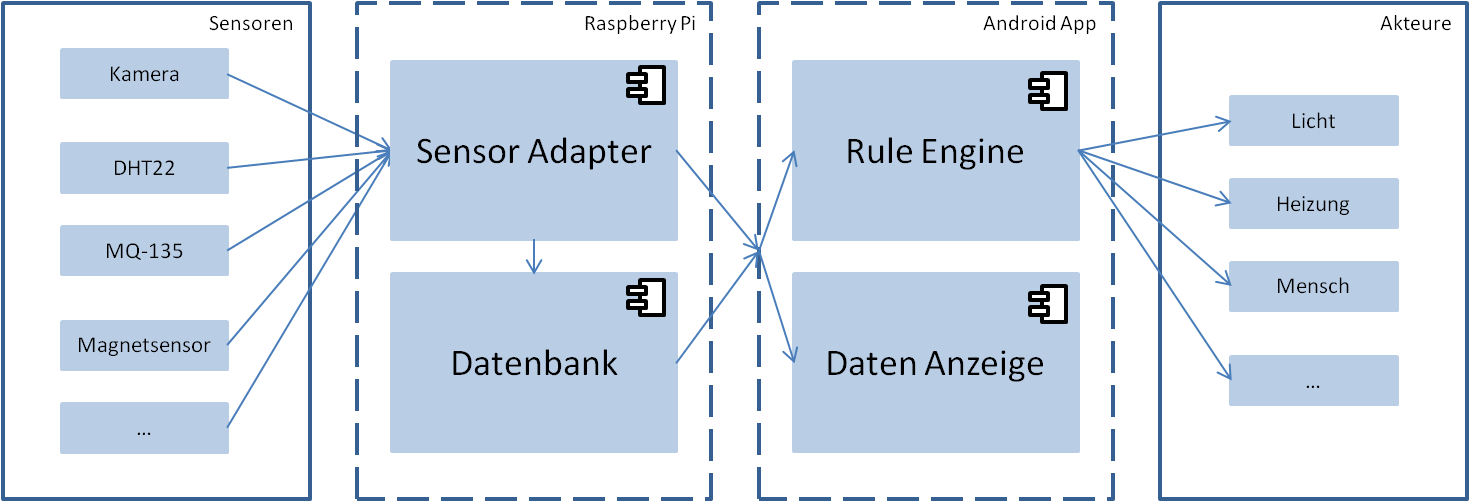
\includegraphics[width=1\textwidth]{images/Konzept_allgemein.png}
	\caption{Kontextsicht Soll-Zustand}
	\label{fig:M1}
\end{figure}
Aufbauend auf das erstellte Konzept wird die Architektur des Systems entworfen. Im folgenden Kapitel wird auf die einzelnen Komponenten im Genauen eingegangen und wie diese im Kontext dieser Arbeit optimal umgesetzt werden. 